
% --- SLIDE 6: LABEL LAG ---
\begin{frame}{The Label-Lag Problem}

    \centering
    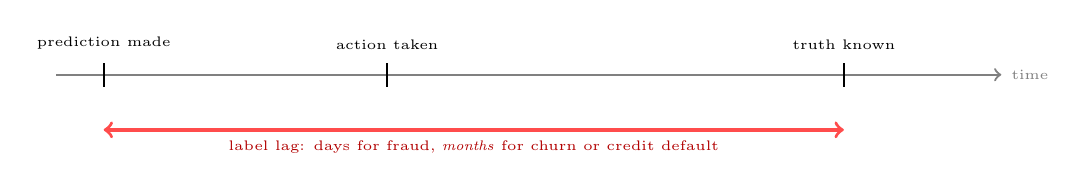
\begin{tikzpicture}[font=\scriptsize]
        \draw[->, thick, gray] (0,0) -- (12.0,0) node[right, font=\tiny] {time};
        \foreach \x/\lab in {0.6/{prediction made}, 4.2/{action taken}, 10.0/{truth known}} {
            \draw[thick] (\x,-0.15) -- (\x,0.15);
            \node[anchor=south, font=\tiny, align=center] at (\x,0.2) {\lab};
        }
        \draw[<->, very thick, red!70] (0.6,-0.7) -- node[below, font=\tiny, red!70!black]
            {label lag: days for fraud, \emph{months} for churn or credit default} (10.0,-0.7);
    \end{tikzpicture}

    \vspace{1.0em}
    \begin{itemize}
        \item You cannot compute accuracy in production until the labels arrive. For a 12-month loan default
              model, that is a \textbf{12-month} feedback delay.
        \item \textbf{Proxies to use in the meantime:}
              \begin{itemize}
                  \item input and prediction distribution monitoring (previous slide);
                  \item \textbf{business metrics} that respond faster --- click-through, override rate,
                        complaint volume, manual-review queue length;
                  \item \textbf{human spot-checks}: label a small random sample every week, deliberately.
                        A hundred labels a week is a real accuracy estimate.
              \end{itemize}
        \item \textbf{Beware biased feedback:} if you only ever see the outcome for applicants you approved,
              your production ``accuracy'' is measured on a censored sample.
    \end{itemize}

\end{frame}
